\documentclass[12pt, a4paper]{article}
\usepackage{fullpage}
\usepackage{amsmath}
\usepackage{graphicx}
\usepackage{natbib}
\title{Implementation of CLM Below-Ground Biogeochemistry in PFLOTRAN}
%\author{Guoping Tang}
\date\today{}

\begin{document}
\maketitle

\begin{abstract}
\end{abstract}

\section{CLM-CN}
\subsection{Reactions}
\begin{figure}[h]
\centering
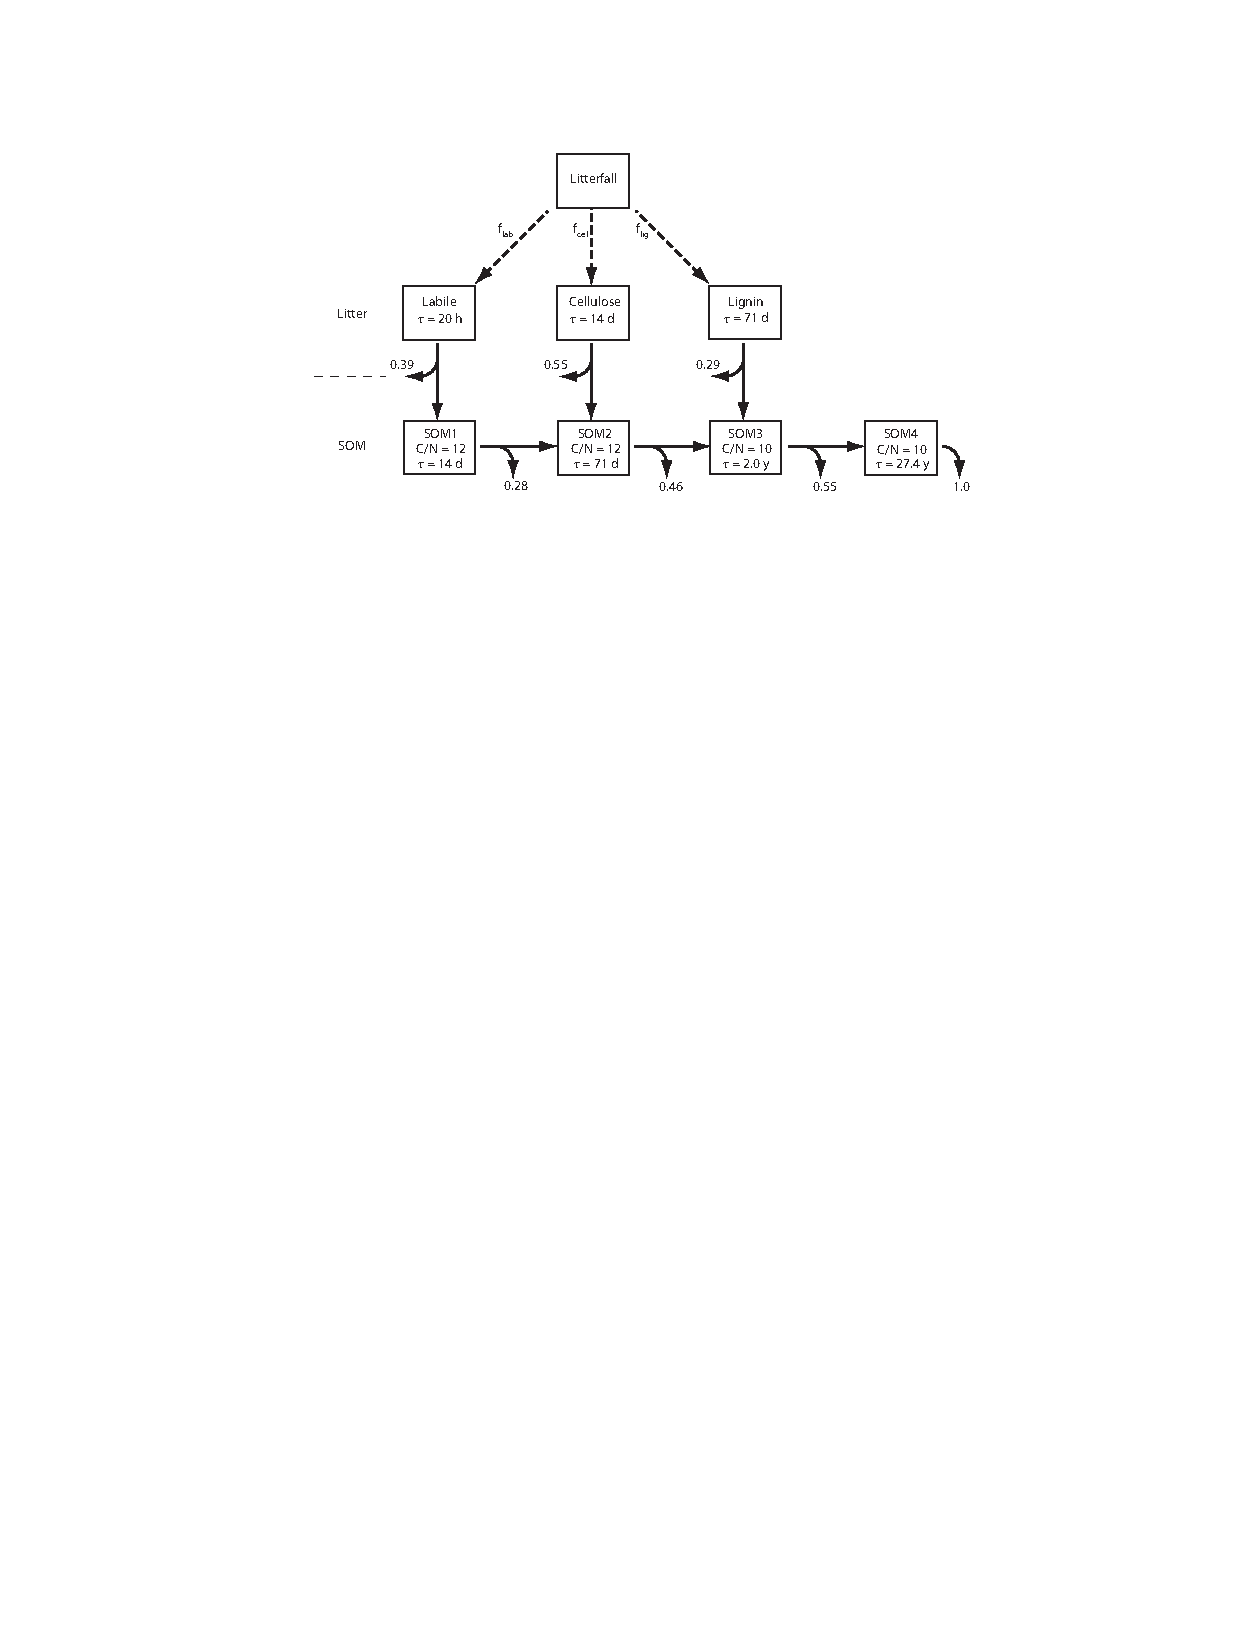
\includegraphics[width=1.0\textwidth]{Bonan.pdf}
\caption{CLM-CN litter and soil organic pools and C and N flows \cite{Bonanetal2012}}
\label{Fig1}
\end{figure}

\subsubsection{General Reaction}
The general decomposition reaction is
\begin{equation}
\label{rxnclmcn}
\text{CN}_u = (1 - f) \text{CN}_d + f \text{CO}_2 + n \text{N}_\text{mineral}
\end{equation}

\begin{tabular}{lll}
$\text{CN}_u$ & = & upstream pool [mol/m$^3$] \\
$\text{CN}_d$ & = & downstream pool [mol/m$^3$] \\
$\text{CO}_2$ & = & [mol/m$^3$] \\
$\text{N}_\text{mineral}$ & = &mineral nitrogen [mol/m$^3$] \\
$u$ & = & molecular weight ratio of C and N divided by upstream pool C/N [-]\\
$d$ & = & molecular weight ratio of C and N divided by downstream pool C/N [-]\\
$f$ & = & respiration fraction [-] \\
$n$ & = & $[u - (1 - f)d]$
\end{tabular}

\subsubsection{Soil Organic Matter Pools}
The C/N ratio is fixed in soil organic matter pools. The reactions are

\begin{table}[h]
\caption{Reactions for the soil organic matter pools}
\begin{center}
\begin{tabular}{lll}
SOM1 & = & 0.72 SOM2 + 0.28 $\text{CO}_2$ + 0.020000 $\text{N}_ \text{mineral}$ \\
SOM2 & = & 0.54 SOM3 + 0.46 $\text{CO}_2$ + 0.025143 $\text{N}_\text{mineral}$  \\
SOM3 & = & 0.45 SOM4 + 0.55 $\text{CO}_2$ + 0.047143 $\text{N}_ \text{mineral}$ \\
SOM4 & = & $\text{CO}_2$ + 0.085714 $\text{N}_\text{mineral}$  
\end{tabular}
\end{center}
\label{SOMReactions}
\end{table}

\subsubsection{Litter Pools}
The C/N ratio is dependent on the input from plant function groups. As the C/N ratio is generally greater in the litter pools than in the soil organic pools \cite{Adairetal2008}, mineral N is needed to decompose the litter pools. Namely, litter decomposition involves N immobilization through microbial mass synthesis. For example, one observation indicates a C/N ratio of 31.19 for yellow birch \cite{Adairetal2008}. The reactions are

\begin{table}[h]
\caption{Reactions for the litter pools}
\begin{center}
\begin{tabular}{lll}
Lit1C + 0.027481 Lit1N + 0.016090 $\text{N}_\text{mineral}$ & = & 0.61 SOM1 + 0.39 $\text{CO}_2$  \\
Lit2C + 0.027481 Lit2N + 0.004662 $\text{N}_\text{mineral}$ & = & 0.45 SOM2 + 0.55 $\text{CO}_2$  \\
Lit3C + 0.027481 Lit3N + 0.033376 $\text{N}_\text{mineral}$ & = & 0.71 SOM3 + 0.29 $\text{CO}_2$  \\
\end{tabular}
\end{center}
\label{LitterReactions}
\end{table}

\subsubsection{Summary}
\begin{align*}
\text{Lit1C} + u_1 \text {Lit1N} & = \left(1-f_1\right) \text{SOM1} + f_1 \text{CO}_2 + n_1 \text{N}_\text{mineral} \\
\text{Lit2C} + u_2 \text {Lit2N} & = \left(1-f_2\right) \text{SOM2} + f_2 \text{CO}_2 + n_2 \text{N}_\text{mineral} \\
\text{Lit3C} + u_3 \text {Lit3N} & = \left(1-f_3\right) \text{SOM3} + f_3 \text{CO}_2 + n_3 \text{N}_\text{mineral} \\
\text{SOM1} & = \left(1-f_4\right) \text{SOM2} + f_4 \text{CO}_2 + n_4 \text{N}_\text{mineral} \\
\text{SOM2} & = \left(1-f_5\right) \text{SOM3} + f_5 \text{CO}_2 + n_5 \text{N}_\text{mineral} \\
\text{SOM3} & = \left(1-f_6\right) \text{SOM4} + f_6 \text{CO}_2 + n_6 \text{N}_\text{mineral} \\
\text{SOM4} & = f_7 \text{CO}_2 + n_7 \text{N}_\text{mineral} \\
\end{align*}

\begin{equation*}
u_i = \text{LitiN}/\text{LitiC}
\end{equation*}

\subsection{Rate}
\subsubsection{General}
\begin{equation}
\label{clmcn_rate}
R = f_T f_\Psi f_\text{N} k \text{CN}_u
\end{equation}

\begin{align*}
R &= \text{rate [mol/(m}^3\text{s)]} \\
f_T & = \exp\left[308.56 \left(\frac{1}{71.02}-\frac{1}{T - 227.13}\right)\right]\\
f_\Psi & = \frac{\log\left(\Psi_\text{min}/\Psi\right)}{\log\left(\Psi_\text{min}/\Psi_\text{max}\right)}\\
f_\text{N} & = \frac{\text{N}_\text{mineral}}{\text{N}_\text{mineral} + k_{\text{N}_\text{mineral}}} (\text{if u} < 0) \\
k & = \text{kinetic rate constant} [\text{s}^{-1}]\\
T & = \text{temperature } [\text{K}] \\
\Psi & = \text{soil water potential} [\text{Pa}] \\
\text{CN}_u & = \text{upstream carbon pool } [\text{mol/m}^3] \\
\text{N}_\text{mineral} & = \text{nitrogen concentration } [\text{mol/m}^3] \\
k_\text{N} & = \text{Mineral N half saturation constant } [\text{mol/m}^3]\\
\end{align*}

For the general reaction \ref{rxnclmcn}, 
\begin{align*}
\frac{\partial \text{CN}_u}{\partial t} & = -R \\
\frac{\partial \text{CN}_d}{\partial t} & = \left(1-f\right) R \\
\frac{\partial \text{CO}_2}{\partial t} & = f R \\
\frac{\partial \text{N}_\text{mineral}}{\partial t} & = nR \\
\end{align*}

\subsubsection{Rates}
\begin{align*}
R_1 = f_T f_\theta f_\text{N} k_1 \text{Lit1C} \\
R_2 = f_T f_\theta f_\text{N} k_2 \text{Lit2C} \\
R_3 = f_T f_\theta f_\text{N} k_3 \text{Lit3C} \\
R_4 = f_T f_\theta f_\text{N} k_4 \text{SOM1} \\
R_5 = f_T f_\theta f_\text{N} k_5 \text{SOM2} \\
R_6 = f_T f_\theta f_\text{N} k_6 \text{SOM3} \\
R_7 = f_T f_\theta f_\text{N} k_7 \text{SOM4}
\end{align*}

\subsubsection{Mass Conservation}
\begin{align*}
\frac{\partial}{\partial t} \left(\text{Lit1C}\right) & =  -R_1 \\
\frac{\partial}{\partial t} \left(\text{Lit1N}\right) & =  -u_1 R_1\\
\frac{\partial}{\partial t} \left(\text{Lit2C}\right) & =  -R_2 \\
\frac{\partial}{\partial t} \left(\text{Lit3N}\right) & =  -u_2 R_2 \\
\frac{\partial}{\partial t} \left(\text{Lit3C}\right) & =  -R_3 \\
\frac{\partial}{\partial t} \left(\text{Lit3N}\right) & =  -u_3 R_3 \\
\frac{\partial}{\partial t} \left(\text{SOM1}\right) & = (1-f_1)R_1 - R_4 \\
\frac{\partial}{\partial t} \left(\text{SOM2}\right) & = (1-f_2)R_2 + (1-f_4)R_4 - R_5 \\
\frac{\partial}{\partial t} \left(\text{SOM3}\right) & = (1-f_3)R_3 + (1-f_5)R_5 - R_6 \\
\frac{\partial}{\partial t} \left(\text{SOM4}\right) & = (1-f_6)R_6 - R_7  \\
\frac{\partial}{\partial t} \left(\text{CO}_2\right) & =  f_1R_1 + f_2R_2 + f_3R_3 + f_4R_4 + f_5R_5 + f_6R_6 + f_7R_7 \\
\frac{\partial}{\partial t} \left(\text{N}_\text{mineral}\right) & = n_1R_1 + n_2R_2 + n_3R_3 +n_4R_4 +n_5R_5 +n_6R_6 + n_7R_7 \\
\end{align*}

\subsection{Implementation in PFLOTRAN}
\subsubsection{Numerical Methods}
Applying finite-volume spatial discretization:
\begin{equation}
\int \frac{\partial x}{\partial t} dV =  \int -\sum R_j dV
\end{equation}

\begin{equation}
\frac{\partial x}{\partial t} \Delta V = - \sum R_j \Delta V
\end{equation}

Implicit time discretization:
\begin{equation}
\frac{\Delta V}{\Delta t} \left(x^{k+1} - x^k\right) = - \sum R_j^{k+1} \Delta V
\end{equation}

Residual:
\begin{equation}
\mathcal{R} = \frac{\Delta V}{\Delta t} \left(x^{k+1} - x^k\right)  + \sum R_i^{k+1} \Delta V
\end{equation}

Jacobian:
\begin{equation}
\mathcal{J} =\frac{\partial \mathcal{R}}{\partial x}
\end{equation}


Newton-Raphson Method:
\begin{equation}
\mathcal{J} \delta x = -\mathcal{R}
\end{equation}

\begin{equation}
x^{k+1,i+1} = x^{k+1,i}+ \delta x
\end{equation}

\begin{table}[h]
\caption{Units for residuals and Jacobian}
\begin{center}
\begin{tabular}{ccccc}
                             & aqueous species & immobile species & mixed\\
$x$                      &  mol/L      & mol/m$^3$ &   \\               
$\Delta V$          &  L   & m$^3$  & L \\
$R$                     &  mol/Ls & mol/m$^3$s  & mol/Ls \\
$\mathcal{R}$   & mol/s       & mol/s & mol/s \\ 
$\mathcal{J}$    & L/s & m$^3$/s & \\
\end{tabular}
\end{center}
\label{units}
\end{table}

\subsubsection{Implementation}
The source code reaction\_sandbox\_clm\_cn.F90 implements CLM-CN with input file like the following: 

\begin{verbatim}
CHEMISTRY
  ...
  IMMOBILE_SPECIES
    N
    C
    SOM1
    SOM2
    SOM3
    SOM4
    LabileC
    CelluloseC
    LigninC
    LabileN
    CelluloseN
    LigninN
  /
  ...
  REACTION_SANDBOX
    CLM-CN
      POOLS   ! CN ratio
        SOM1  12.d0
        SOM2  12.d0
        SOM3  10.d0
        SOM4  10.d0
        Labile
        Cellulose
        Lignin
      /
      REACTION
        UPSTREAM_POOL Labile
        DOWNSTREAM_POOL SOM1
        TURNOVER_TIME 20. h
        RESPIRATION_FRACTION 0.39d0
        N_INHIBITION 1.d-10
      /
      REACTION
        UPSTREAM_POOL Cellulose
        DOWNSTREAM_POOL SOM2
        TURNOVER_TIME 14. d
        RESPIRATION_FRACTION 0.55
        N_INHIBITION 1.d-10
      /
      REACTION
        UPSTREAM_POOL Lignin
        DOWNSTREAM_POOL SOM3
        TURNOVER_TIME 71. d
        RESPIRATION_FRACTION 0.29d0
        N_INHIBITION 1.d-10
      /
      REACTION
        UPSTREAM_POOL SOM1
        DOWNSTREAM_POOL SOM2
        TURNOVER_TIME 14. d
        RESPIRATION_FRACTION 0.28d0
        N_INHIBITION 1.d-10
      /
      REACTION
        UPSTREAM_POOL SOM2
        DOWNSTREAM_POOL SOM3
        TURNOVER_TIME 71. d
        RESPIRATION_FRACTION 0.46d0
        N_INHIBITION 1.d-10
      /
      REACTION
        UPSTREAM_POOL SOM3
        DOWNSTREAM_POOL SOM4
        TURNOVER_TIME 2. y
        RESPIRATION_FRACTION 0.55d0
        N_INHIBITION 1.d-10
      /
      REACTION
        UPSTREAM_POOL SOM4
        TURNOVER_TIME 27.4 y
        RESPIRATION_FRACTION 1.d0
        N_INHIBITION 1.d-10
      /
    /
  /
\end{verbatim}
In the source code, the key is to specify the residual and Jacobian. The residuals are:
\begin{align*}
\mathcal{R}_{\text{Lit1C}} & = \frac{\Delta V}{\Delta t} \left(\text{Lit1C}^{k+1} - \text{Lit1C}^k\right)  + R_1^{k+1} \Delta V \\
\mathcal{R}_{\text{Lit1N}} & = \frac{\Delta V}{\Delta t} \left(\text{Lit1N}^{k+1} - \text{Lit1N}^k\right)  + u_1 R_1^{k+1} \Delta V \\
\mathcal{R}_{\text{Lit2C}} & = \frac{\Delta V}{\Delta t} \left(\text{Lit2C}^{k+1} - \text{Lit2C}^k\right)  + R_2^{k+1} \Delta V \\
\mathcal{R}_{\text{Lit2N}} & = \frac{\Delta V}{\Delta t} \left(\text{Lit2N}^{k+1} - \text{Lit2N}^k\right)  + u_2 R_2^{k+1} \Delta V \\
\mathcal{R}_{\text{Lit3C}} & = \frac{\Delta V}{\Delta t} \left(\text{Lit3C}^{k+1} - \text{Lit3C}^k\right)  + R_3^{k+1} \Delta V \\
\mathcal{R}_{\text{Lit3N}} & = \frac{\Delta V}{\Delta t} \left(\text{Lit3N}^{k+1} - \text{Lit3N}^k\right)  + u_3 R_3^{k+1} \Delta V \\
\mathcal{R}_{\text{SOM1}} & = \frac{\Delta V}{\Delta t} \left(\text{SOM1}^{k+1} - \text{SOM1}^k\right)  - \left[ (1 - f_1) R_1^{k+1} - R_4^{k+1} \right] \Delta V \\
\mathcal{R}_{\text{SOM2}} & = \frac{\Delta V}{\Delta t} \left(\text{SOM2}^{k+1} - \text{SOM2}^k\right)  - \left[ (1 - f_2) R_2^{k+1} + (1 - f_4) R_4^{k+1} - R_5^{k+1} \right] \Delta V \\
\mathcal{R}_{\text{SOM3}} & = \frac{\Delta V}{\Delta t} \left(\text{SOM3}^{k+1} - \text{SOM3}^k\right)  - \left[ (1 - f_3) R_3^{k+1} + (1 - f_5) R_5^{k+1} - R_6^{k+1} \right] \Delta V \\
\mathcal{R}_{\text{SOM4}} & = \frac{\Delta V}{\Delta t} \left(\text{SOM4}^{k+1} - \text{SOM4}^k\right)  - \left[ (1 - f_6) R_6^{k+1} - R_7^{k+1} \right] \Delta V \\
\mathcal{R}_{\text{CO}_\text{2}} & = \frac{\Delta V}{\Delta t} \left(\text{CO}_\text{2}^{k+1} - \text{CO}_\text{2}^k\right)  \\
  & - \left[f_1R_1^{k+1} + f_2R_2^{k+1} + f_3R_3^{k+1} + f_4R_4^{k+1} + f_5R_5^{k+1} + f_6R_6^{k+1} + R_7^{k+1}\right]\Delta V \\
\mathcal{R}_{\text{N}_\text{mineral}} & = \frac{\Delta V}{\Delta t} \left(\text{N}_\text{mineral}^{k+1} - \text{N}_\text{mineral}^k\right) \\
  & - \left[n_1R_1^{k+1} + n_2R_2^{k+1} + n_3R_3^{k+1} + n_4R_4^{k+1} + n_5R_5^{k+1} + n_6R_6^{k+1} + R_7^{k+1}\right]\Delta V  
\end{align*}
 
For Lit1 decomposition, the rate is

\begin{equation}
R_1 = f_T f_\Psi f_\text{N} k_1 \text{Lit1C} 
\end{equation}

the derivatives are:
\begin{equation}
\frac{\partial R_1}{\partial \text{Lit1C}} = f_T f_\Psi f_\text{N} k_1 = R'_\text{1,Lit1C}
\end{equation}

\begin{equation}
\frac{\partial R_1}{\partial \text{N}_\text{mineral}} = f_T f_\Psi k_1 \text{Lit1C} \frac{k_N}{(k_N + \text{N}_\text{mineral})^2} = R'_\text{1,N}
\end{equation}

\begin{tabular}{ llll}
$\frac{\partial R_\text{Lit1N}}{\partial \text{Lit1C}}$ &= $\frac{\partial (u_1R_1)}{\partial \text{Lit1C}}$ &= $R_1 \frac{\partial u_1}{\partial \text{Lit1C}}+ u_1R_\text{1,Lit1C}$ &= $-R_1 \frac{\text{Lit1N}}{ \text{Lit1C}^2}+ u_1R'_\text{1,Lit1C}$  \\
$\frac{\partial R_\text{Lit1N}}{\partial \text{Lit1N}}$ &= $\frac{\partial (u_1R_1)}{\partial \text{Lit1N}}$ &= $R_1 \frac{\partial u_1}{\partial \text{Lit1N}}$ &= $R_1 \frac{1}{ \text{Lit1C}} $\\ 
$\frac{\partial R_\text{Lit1N}}{\partial \text{Nmineral}}$ &= $\frac{\partial (u_1R_1)}{\partial \text{Nmineral}}$ &= $R_1 \frac{\partial u_1}{\partial \text{Nmineral}} + u_1 R'_\text{1,N}$ &= $u_1R'_\text{1,N}$  \\
$\frac{\partial R_\text{Nmineral}}{\partial \text{Lit1C}}$ &= $-\frac{\partial (n_1R_1)}{\partial \text{Lit1C}}$ &= $-R_1 \frac{\partial n_1}{\partial \text{Lit1C}}- n_1R'_\text{1,Lit1C}$ &= $R_1 \frac{\text{Lit1N}}{ \text{Lit1C}^2} - n_1R'_\text{1,Lit1C} $ \\
$\frac{\partial R_\text{Nmineral}}{\partial \text{Lit1N}}$ &= $-\frac{\partial (n_1R_1)}{\partial \text{Lit1N}}$ &= $-R_1 \frac{\partial n_1}{\partial \text{Lit1N}}$ &= $-R_1 \frac{1}{ \text{Lit1C}}$ \\
$\frac{\partial R_\text{Nmineral}}{\partial \text{N}_\text{mineral}}$ &= $-\frac{\partial (n_1R_1)}{\partial \text{N}_\text{mineral}}$ & = $-R_1 \frac{\partial n_1}{\partial \text{N}_\text{mineral}}$ &= $-n_1R'_{1,N}$  \\
\end{tabular}

\begin{table}[hb]
\centering
 \caption{Jacobian for Litter Pools} 
\begin{tabular}{ c | ccccc }
                                              &  LitiC  & LitiN & SOMi & $\text{CO}_\text{2}$ & $\text{N}_\text{mineral}$ \\
  \hline
  LitiC                                   & $R'_\text{i,LitiC}$ & 0 & 0 & 0 & $R'_{i,N} $ \\
  LitiN                                   &  $-R_i \frac{\text{LitiN}}{ \text{LitiC}^2}+ u_iR'_\text{i,LitiC} $ & $R_i \frac{1}{ \text{LitiC}} $  &0  & 0 & $u_i R'_{i,N}$  \\
  SOMi                                 & $-(1-f_i)R'_\text{i,LitiC}$ & 0 & 0 & 0 & $-(1-f_i)R'_{i,N} $  \\
  $\text{CO}_\text{2}$         & $-f_iR'_\text{i,LitiC}$ & 0 & 0 & 0 & $-f_iR'_{i,N} $  \\
  $\text{N}_\text{mineral}$ & $R_i \frac{\text{LitiN}}{ \text{LitiC}^2} - n_iR'_\text{i,LitiC} $  & $-R_1 \frac{1}{ \text{LitiC}}$ & 0 & 0 & $-n_i R'_{i,N}$ \\
\end{tabular}
\end{table}

\begin{table}[hb]
\centering
 \caption{Jacobian for SOM Pools} 
\begin{tabular}{ c | cccccc }
                                              &  SOM1  & SOM2 & SOM3 & SOM4 & $\text{CO}_\text{2}$ & $\text{N}_\text{mineral}$ \\
  \hline
  SOM1                                 & $R'_4$ & 0 & 0 & 0 & 0 & 0 \\
  SOM2                                 &  $-(1-f_4)R'_4$ & $R'_5$  &0  & 0 & 0 & 0  \\
  SOM3                                 & 0 & $-(1-f_5)R'_5$ & $R'_6$ & 0 & 0  & 0 \\
  SOM4                                 & 0 & 0 & $-(1-f_6)R'_6$ & $R'_7$ & 0  & 0 \\
  $\text{CO}_\text{2}$         & $-f_4R'_4$ & $-f_5R'_5$ & $-f_6R'_6$  & $-R'_7$ & 0  & 0 \\
  $\text{N}_\text{mineral}$ & $-n_4R'_4$  & $-n_5R'_5$ & $-n_6R'_6$ & $-n_7R'_7$ & 0 & 0 \\
\end{tabular}
\end{table}

\subsection{Applications}
\begin{figure}[h]
\centering
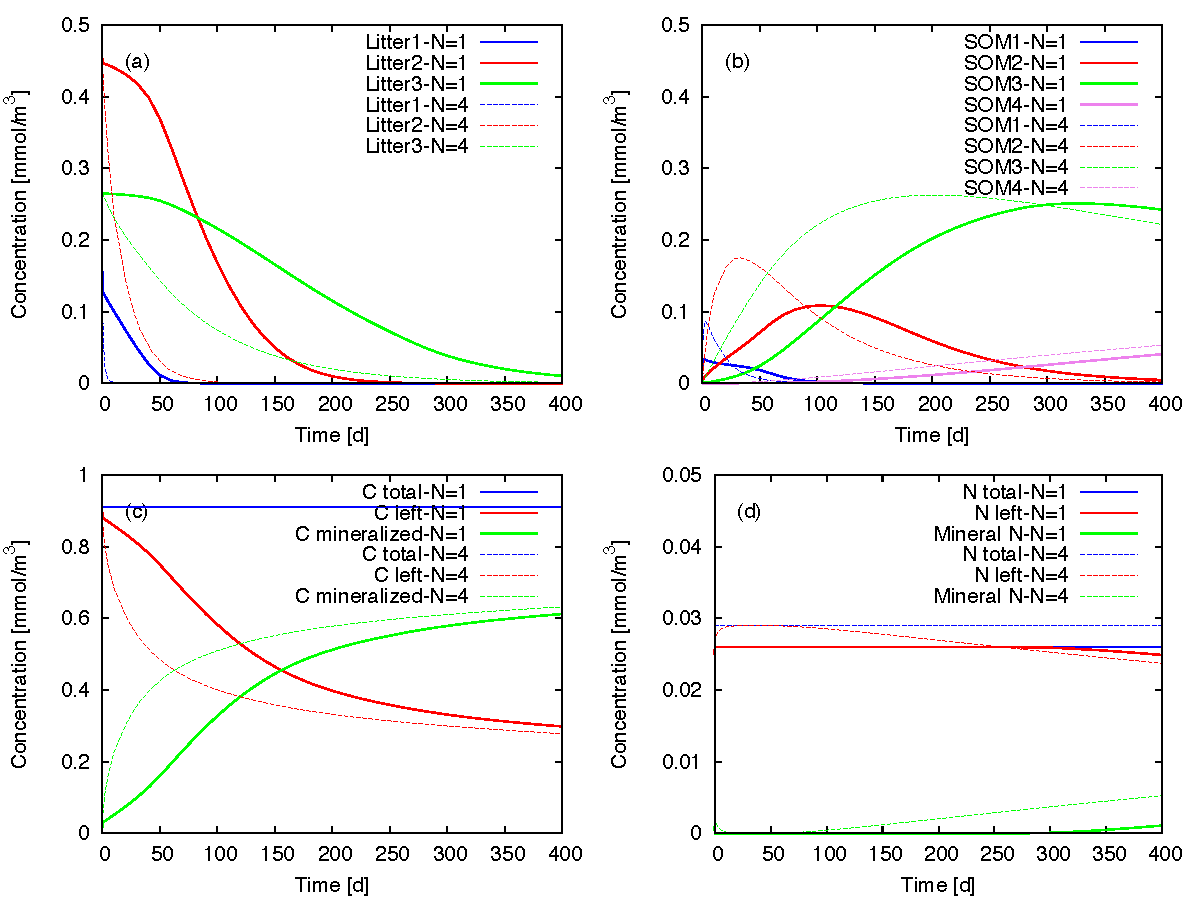
\includegraphics[width=1.0\textwidth]{../CLM-CN/comp.pdf}
\caption{Demonstrating N limiting on C decomposition (initial mineral N=1 and 4 $\mu$ mol/m$^3$)}
\label{Fig2}
\end{figure}

%\newpage
\clearpage
\section{CLM4.5 CH$_4$ Oxidation}
\subsection{Reaction}
\begin{equation}
\label{rxnclm45ch4o}
\text{CH}_4 + 2 \text{O}_2 =  \text{CO}_2 + 2 \text{H}_2\text{O}
\end{equation}

\subsection{Rate}
\begin{equation}
\label{clm45ch4orate}
R =  k \frac{\text{CH}_4}{k_\text{CH4} + \text{CH}_4} \frac{\text{O}_2}{k_\text{O2} + \text{O}_2} f_T f_\Psi
\end{equation}

\subsection{Residuals}
\begin{align*}
\mathcal{R}_{\text{CH4}} & = \frac{\Delta V}{\Delta t} \left(\text{CH}_4^{k+1} - \text{CH}_4^k\right)  + R^{k+1} \Delta V \\
\mathcal{R}_{\text{O2}} & = \frac{\Delta V}{\Delta t} \left(\text{O}_2^{k+1} - \text{O}_2^k\right)  + 2 R^{k+1} \Delta V \\
\mathcal{R}_{\text{CO2}} & = \frac{\Delta V}{\Delta t} \left(\text{CO}_2^{k+1} - \text{CO}_2^k\right)  - R^{k+1} \Delta V \\
\end{align*}

\subsection{Jacobian}

\begin{align*}
\frac{\partial R}{\partial \text{CH}_4} &= k \frac{k_\text{CH4}}{(k_\text{CH4} + \text{CH}_4)^2} \frac{\text{O}_2}{k_\text{O2} + \text{O}_2} f_T f_\Psi = R'_\text{CH4} \\
\frac{\partial R}{\partial \text{O}_2} &= k \frac{\text{CH}_4}{k_\text{CH4} + \text{CH}_4} \frac{k_\text{O2}}{(k_\text{O4} + \text{O}_2)^2}  f_T f_\Psi = R'_\text{O2} \\
\end{align*}

\begin{table}[hb]
\centering
 \caption{Jacobian for methane oxidation} 
\begin{tabular}{ c | ccc }
                      &  CH$_4$  & O$_2$ &  CO$_2$ \\
  \hline
  CH$_4$     & $R'_\text{CH4}$ & $R'_\text{O2}$ & 0 \\
  O$_2$        & $2R'_\text{CH4}$ & $2R'_\text{O2}$ & 0 \\
  CO$_2$     & $-R'_\text{CH4}$ & $-R'_\text{O2}$ & 0 \\
\end{tabular}
\end{table}



\subsection{Application}
Input file
\begin{verbatim}
CHEMISTRY
  PRIMARY_SPECIES
    O2(aq)
    Methane(aq)
    CO2(aq)
  /
  REDOX_SPECIES
    CO2(aq)
    Methane(aq)
    O2(aq)
  /
  REACTION_SANDBOX
    CH4O
      RATE_CONSTANT 1.25d-10 ! mol/m3 s
      HALFSATURATIONCH4 5.0d-6
      HALFSATURATIONO2  2.0d-5
    /
  /
  DATABASE ../../pflotran-clm4me/database/hanford.dati
......
CONSTRAINT initial
  CONCENTRATIONS
    O2(aq)      0.001 T
    Methane(aq) 0.001 T
    CO2(aq)   1.0d-10 T
  /
END
\end{verbatim}

Code
\begin{verbatim}
subroutine CH4OReact(this,Residual,Jacobian,compute_derivative, &
                         rt_auxvar,global_auxvar,porosity,volume,reaction, &
                         option)
  word = "Methane(aq)"
  is_ch4 = GetPrimarySpeciesIDFromName(word,reaction,option)
 
  word = "CO2(aq)"
  is_co2 = GetPrimarySpeciesIDFromName(word,reaction,option)

  word = "O2(aq)"
  is_o2 = GetPrimarySpeciesIDFromName(word,reaction,option)
 
  temp_K = global_auxvar%temp(1) + 273.15d0
  F_t = exp(308.56d0*(one_over_71_02 - 1.d0/(temp_K - 227.13d0)))
 
  F_theta = log(theta_min/global_auxvar%sat(1)) * one_over_log_theta_min
 
  L_water = porosity*global_auxvar%sat(iphase)*volume*1.d3
  c_ch4 = rt_auxvar%total(is_ch4,iphase) 
  c_o2 = rt_auxvar%total(is_o2,iphase)   

  rate = this%rate_constant * L_water * &  ! mole/(L sec)
    c_ch4/(this%kmch4 + c_ch4) * c_o2/(this%kmo2 + c_o2) * F_t * F_theta

  Residual(is_ch4) = Residual(is_ch4) + rate
  Residual(is_o2) = Residual(is_o2) + 2.0 * rate
  Residual(is_co2) = Residual(is_co2) - rate
 
  if (compute_derivative) then

    ! always add contribution to Jacobian
    ! units = (mol/sec)*(kg water/mol) = kg water/sec
  
    !dx/(k+x) = k/(k+x)^2
 
    drate_dch4 = rate * this%kmch4 / c_ch4 / (this%kmch4 + c_ch4)
    drate_do2  = rate * this%kmo2 / c_o2 / (this%kmo2 + c_o2)
 
    Jacobian(is_ch4,is_ch4) = Jacobian(is_ch4,is_ch4) - drate_dch4
    Jacobian(is_ch4,is_o2) = Jacobian(is_ch4,is_o2) - drate_do2
    Jacobian(is_o2,is_ch4) = Jacobian(is_o2,is_ch4) - 2.0 * drate_dch4
    Jacobian(is_o2,is_o2) = Jacobian(is_o2,is_o2) - 2.0 * drate_do2
    Jacobian(is_co2,is_ch4) = Jacobian(is_co2,is_ch4) + drate_dch4
    Jacobian(is_co2,is_o2) = Jacobian(is_co2,is_o2) + drate_do2

  endif
 
end subroutine CH4OReact
\end{verbatim}

\begin{figure}[h]
\centering
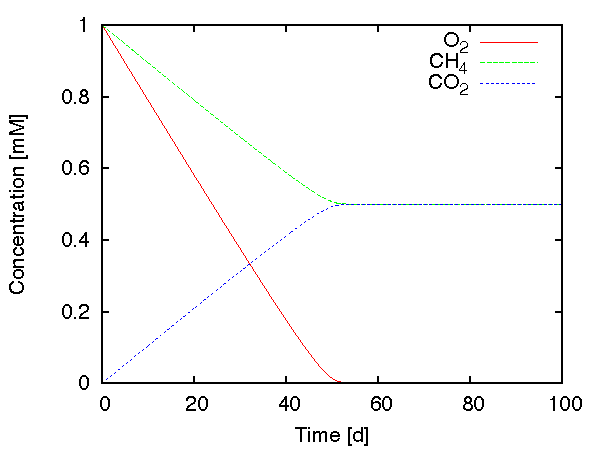
\includegraphics[width=0.6\textwidth]{../ch4oxidation/fig.pdf}
\caption{Example calculation for methane oxidation)}
\label{Fig3}
\end{figure}

\clearpage
\section{Acetoclastic Methanogenesis}
\subsection{Reaction}
\begin{equation}
\label{rxnam}
\text{Ac}^- +  \text{H}_2\text{O} =  \text{CH}_4 + \text{HCO}_3^-
\end{equation}

\begin{equation}
\label{rxnam}
(1 + y/2)\text{Ac}^- +  0.5y \text{H}^+ + \text{H}_2\text{O} =  \text{CH}_4 + \text{HCO}_3^- + y \text{C}_\text{bio}
\end{equation}

\subsection{Rate}
\begin{equation}
\label{amrate}
R =  k \text{C}_\text{bio} \frac{\text{Ac}^-}{k_\text{Ac} + \text{Ac}^-}  f_T f_\Psi
\end{equation}

\subsection{Mass Conservation}
\begin{align*}
\frac{\partial \text{Ac}^-}{\partial t} & = -(1 + \frac{y}{2})R \\
\frac{\partial \text{H}^+}{\partial t} & = -\frac{y}{2}R \\
\frac{\partial \text{CH}_4}{\partial t} & = R \\
\frac{\partial \text{HCO}_3^-}{\partial t} & = R \\
\frac{\partial \text{C}_\text{bio}}{\partial t} & = 1000\theta y R \\
\end{align*}

Note: for the last equation, PFLOTRAN accounts for the $1000\theta$ internally.

\subsection{Residuals}
\begin{align*}
\mathcal{R}_{\text{Ac-}} & = \frac{\Delta V}{\Delta t} \left(\text{Ac}^{-k+1} - \text{Ac}^{-k}\right)  + (1+y/2) R^{k+1} \Delta V \\
\mathcal{R}_\text{CH4} & = \frac{\Delta V}{\Delta t} \left(\text{CH}_4^{k+1} - \text{CH}_4^k\right)  - R^{k+1} \Delta V \\
\mathcal{R}_\text{Cbio} & = \frac{\Delta V}{\Delta t} \left(\text{C}_\text{bio}^{k+1} - \text{C}_\text{bio}^k\right)  - y R^{k+1} \Delta V \\
\mathcal{R}_\text{HCO3-} & = \frac{\Delta V}{\Delta t} \left(\text{HCO}_3^{-k+1} - \text{HCO}_3^{-k}\right)  - R^{k+1} \Delta V \\
\mathcal{R}_\text{H+} & = \frac{\Delta V}{\Delta t} \left(\text{H}^{+k+1} - \text{H}^{+k}\right)  + y/2 R^{k+1} \Delta V \\
\end{align*}

\subsection{Jacobian}

\begin{align*}
\frac{\partial R}{\partial \text{Ac}} &= k \text{C}_\text{bio} \frac{k_\text{Ac}}{(k_\text{Ac} + \text{Ac}^-)^2}  f_T f_\Psi = R'_a \\
\frac{\partial R}{\partial \text{C}_\text{bio}} &= k \frac{\text{Ac}^-}{k_\text{Ac} + \text{Ac}^-}  f_T f_\Psi = R'_b\\
\end{align*}

\begin{table}[hb]
\centering
 \caption{Jacobian for methane oxidation} 
\begin{tabular}{ c | ccccc }
                      &  Ac$^-$ & CH$_4$  & C$_\text{bio}$ &  HCO$_3^-$  & H$^+$\\
  \hline 
  Ac$^-$              &$(1+y/2)R'_a$  & 0 & $(1+y/2)R'_b$   & 0 &0\\
  CH$_4$           &$-R'_a$          & 0 & $-R'_b$  &0 &0\\
  C$_\text{bio}$ &$-yR'_a$       &  0 &$-yR'_b$ &0 &0\\
  HCO$_3^-$     &$-R'_a$         &  0 &$-R'_b$     &0 &0\\
  H$^+$               &$0.5yR'_a$  &  0 &$0.5yR'_b$     &0 &0
\end{tabular}
\end{table}

\subsection{Application}

\noindent Input
\begin{verbatim}
CHEMISTRY
  PRIMARY_SPECIES
    Acetate-
    Methane(aq)
    H+
    HCO3-
  /
  SECONDARY_SPECIES
    OH-
    CO3--
    CO2(aq)
:    Acetic_acid(aq)
  /
  REDOX_SPECIES
    Acetate-
    Methane(aq)
  /
  IMMOBILE_SPECIES
    Acemeg
  /
  REACTION_SANDBOX
     AceMeg
      RATE_CONSTANT      1.0d-6
      HALFSATURATIONAC   1.0d-5
      YIELDCOEFFICIENT   0.02
     /
  /
  DATABASE ../../pflotran-clm4me/database/hanford.dat
/end{verbatim}

\noindent Code
\begin{verbatim} 
  L_water = porosity*global_auxvar%sat(iphase)*volume*1.d3
  c_ac = rt_auxvar%pri_molal(this%is_ac)
  c_bio = rt_auxvar%immobile(this%ispec_id_cbio)

  rate = this%rate_constant * L_water * &
    c_bio * c_ac/(this%kmac + c_ac) * F_t * F_theta

  ! alway subtract contribution from residual (mole/sec)
  Residual(this%is_ac) = Residual(this%is_ac) + (1.0 + 0.5 * this%yield) * rate
  Residual(this%is_ch4) = Residual(this%is_ch4) - rate
  Residual(this%is_cbio) = Residual(this%is_cbio) - this%yield * rate
  Residual(this%is_hco3) = Residual(this%is_hco3) - rate
  Residual(this%is_h) = Residual(this%is_h) + 0.5 * this%yield * rate

  if (compute_derivative) then

! 11. If using an analytical Jacobian, add code for Jacobian evaluation

    ! always add contribution to Jacobian
    ! units = (mol/sec)*(kg water/mol) = kg water/sec

    drate_dac = rate * this%kmac / c_ac / (this%kmac + c_ac)
    drate_dcb = rate / c_bio

    Jacobian(this%is_ac,  this%is_ac)   = Jacobian(this%is_ac,this%is_ac)   &
                                        - (1.0 + 0.5 * this%yield) * drate_dac
    Jacobian(this%is_ch4, this%is_ac)   = Jacobian(this%is_ch4,this%is_ac)  &
                                        + drate_dac
    Jacobian(this%is_cbio,this%is_ac)   = Jacobian(this%is_cbio,this%is_ac) &
                                        + this%yield * drate_dac
    Jacobian(this%is_hco3,this%is_ac)   = Jacobian(this%is_hco3,this%is_ac) &
                                        + 0.5 * this%yield * drate_dac
    Jacobian(this%is_ac,  this%is_cbio) = Jacobian(this%is_ac,this%is_cbio) &
                                        - (1.0 + 0.5 * this%yield) * drate_dcb
    Jacobian(this%is_ch4, this%is_cbio) = Jacobian(this%is_ch4,this%is_cbio) &
                                        + drate_dcb
    Jacobian(this%is_cbio,this%is_cbio) = Jacobian(this%is_cbio,this%is_cbio) &
                                        + this%yield * drate_dcb
    Jacobian(this%is_hco3,this%is_cbio) = Jacobian(this%is_hco3,this%is_cbio) &
                                        + 0.5 * this%yield * drate_dcb

  endif
\end{verbatim}


For  $k_{Ac} = 0$, 
\begin{align*}
\frac{\partial \text{Ac}}{\partial t} &= -(1 + 0.5y) k \text{C}_\text{bio} \\
\frac{\partial \text{C}_\text{bio}}{\partial t} &= 1000\theta y k \text{C}_\text{bio} \\
\end{align*}

\begin{align*}
\text{C}_\text{bio} &= \text{C}_\text{bio,0} \text{EXP}(1000\theta ykt) \\
\text{Ac} &= \text{Ac}_0 - \frac{1+0.5y}{1000\theta y}\text{C}_\text{bio,0} \text{EXP}(1000\theta ykt)  \\
\end{align*}

This analytical solution is used in the following figure to check the numerical solution. Note $\text{C}_\text{bio}$ is supposed to stop increasing when acetate is exhausted. 

\begin{figure}[h]
\centering
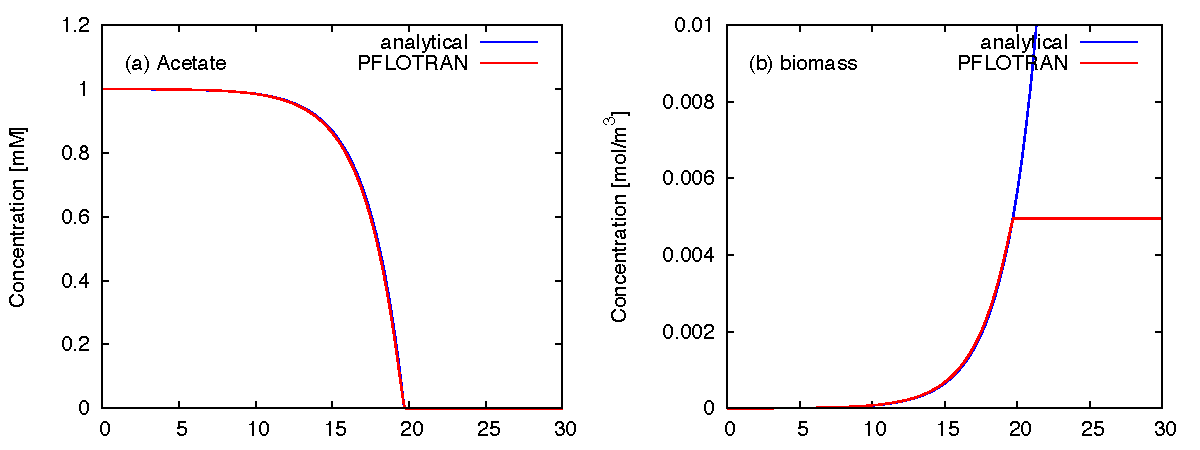
\includegraphics[width=1.0\textwidth]{../acemeg/fig.pdf}
\caption{Example calculation for acetoclastic methanogenesis: }
\label{Fig4}
\end{figure}

\clearpage
\section{Generalization}
If we implement a number of general reactions and rate formulae in PFLOTRAN, we can add as many specific reactions with specific parameter values in the input file. By doing this, we do not have to change the source code or develop a new reaction\_sandbox. For example, if we consider decomposition of LabileC as a first order decay to produce acetate and H$_2$, which are used by methanogens to produce methane using the following reactions:

LabileC = $\frac{1}{3}$ Acetate$^-$ + $\frac{1}{3}$ HCO$_3^-$ + $\frac{1}{9}$ H$_2$ + $\frac{2}{3}$ H$^+$

Acetate$^-$ + H$_2$O = Methane + HCO$_3^-$

H$_2$ + $\frac{1}{4}$ HCO$_3^-$ + $\frac{1}{4}$  H$^+$ = $\frac{1}{4}$ Methane + $\frac{3}{4}$ H$_2$O

We can use the GENERAL\_REACTION and MICROBIAL\_REACTION functions in PFLOTRAN to specify the reactions and parameter values as follow:

\begin{verbatim}
CHEMISTRY
  PRIMARY_SPECIES
    A(aq)
    Acetate-
    H2(aq)
    H+
    HCO3-
    Methane(aq)
    Na+
  /
  SECONDARY_SPECIES
    OH-
    CO3--
    CO2(aq)
:    Acetic_acid(aq)
  /
  REDOX_SPECIES
    Acetate-
    Methane(aq)
    H2(aq)
    H+
  /
  IMMOBILE_SPECIES
    Acmeg
    H2meg
  /

  GENERAL_REACTION
    REACTION A(aq) <-> 0.3333 Acetate- + 0.3333 HCO3- + 0.1111 H2(aq) + 0.6666 H+
    FORWARD_RATE 1.3889d-5  ! 1/s  
    BACKWARD_RATE 0.d0
  /

  MICROBIAL_REACTION
    REACTION Acetate- + H2O <-> Methane(aq) + HCO3-
    RATE_CONSTANT     1.0d-6
    MONOD Acetate-    1.0d-5
    BIOMASS           Acmeg 0.01
  /

  MICROBIAL_REACTION
    REACTION H2(aq) + 0.25 HCO3- + 0.25 H+ <-> 0.25 Methane(aq) + 0.75 H2O
    RATE_CONSTANT     1.0d-5
    MONOD H2(aq)      1.0d-7
    BIOMASS           H2meg 0.02
  /

  DATABASE ../../pflotran-clm4me/database/hanford.dat
\end{verbatim}

With initial conditions as follow,

\begin{verbatim}
CONSTRAINT initial
  CONCENTRATIONS
    A(aq)         0.001 T
    Acetate-    1.0d-10 T
    H2(aq)      1.0d-10 T
    H+              7.0 pH   
    HCO3-        5.0d-3 T
    Methane(aq) 1.0d-10 T
    Na+          5.0d-3 Z
  /
  IMMOBILE
    Acemeg       1.0d-5
    H2meg        1.0d-7
  /
END
\end{verbatim}

PFLOTRAN will give results like in the following figure. The point is that we can add many reactions in the input file.

\begin{figure}[h]
\centering
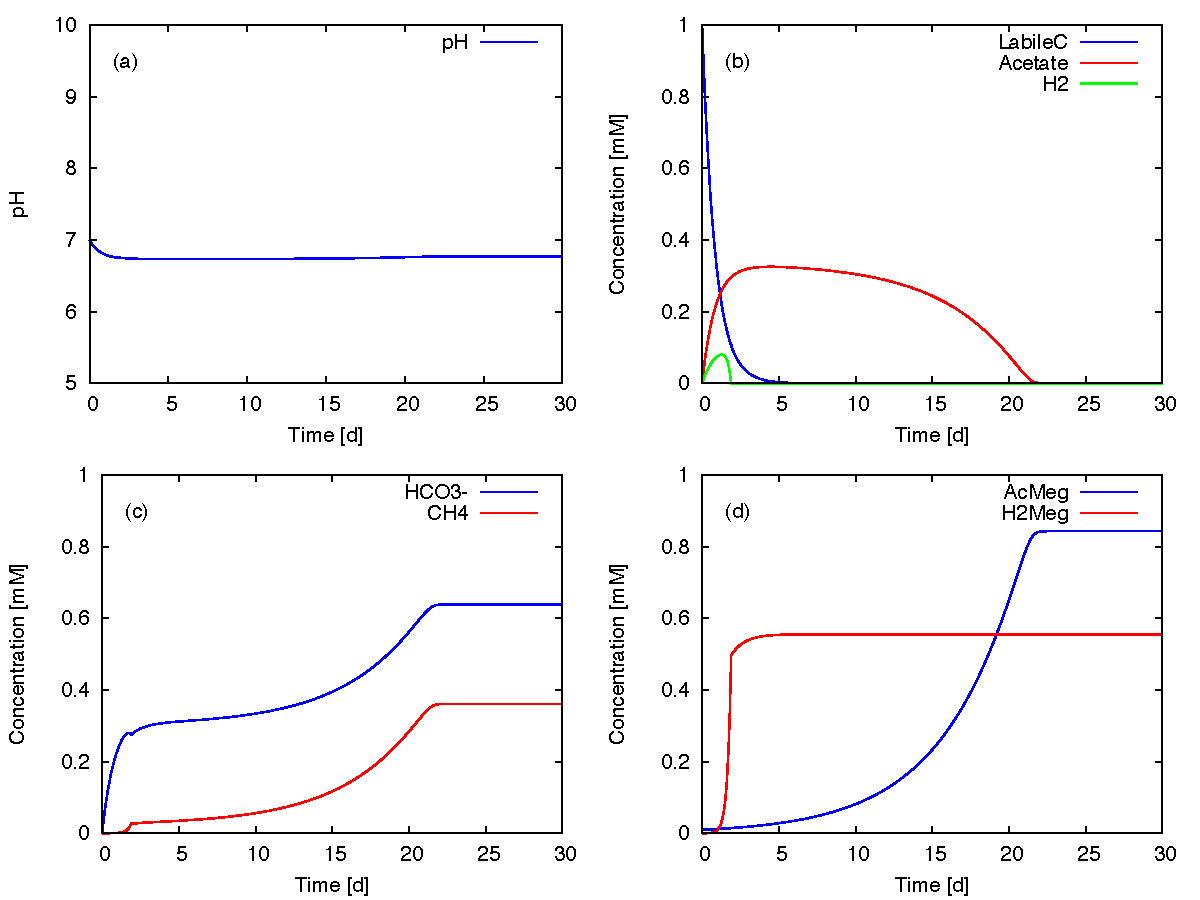
\includegraphics[width=1.0\textwidth]{../microbial/comp.pdf}
\caption{Example calculation for multiple microbial reactions}
\label{Fig5}
\end{figure}






\clearpage
\bibliographystyle{plainnat}
\bibliography{ref}

\end{document}
